\section{Data Integration and Assimilation Systems}
\label{se:dias}

\section{Meteorological Assimilation Data Ingest System}
\label{se:madis}
\acrfull{madis} is a data ingest and assimilation system, which is collecting data over dozen of providers, then quality control over the data and store in \acrshort{netCDF} format. Later allow users to access the data via supporting different type of protocols.

\begin{figure}[htp]
    \centering
    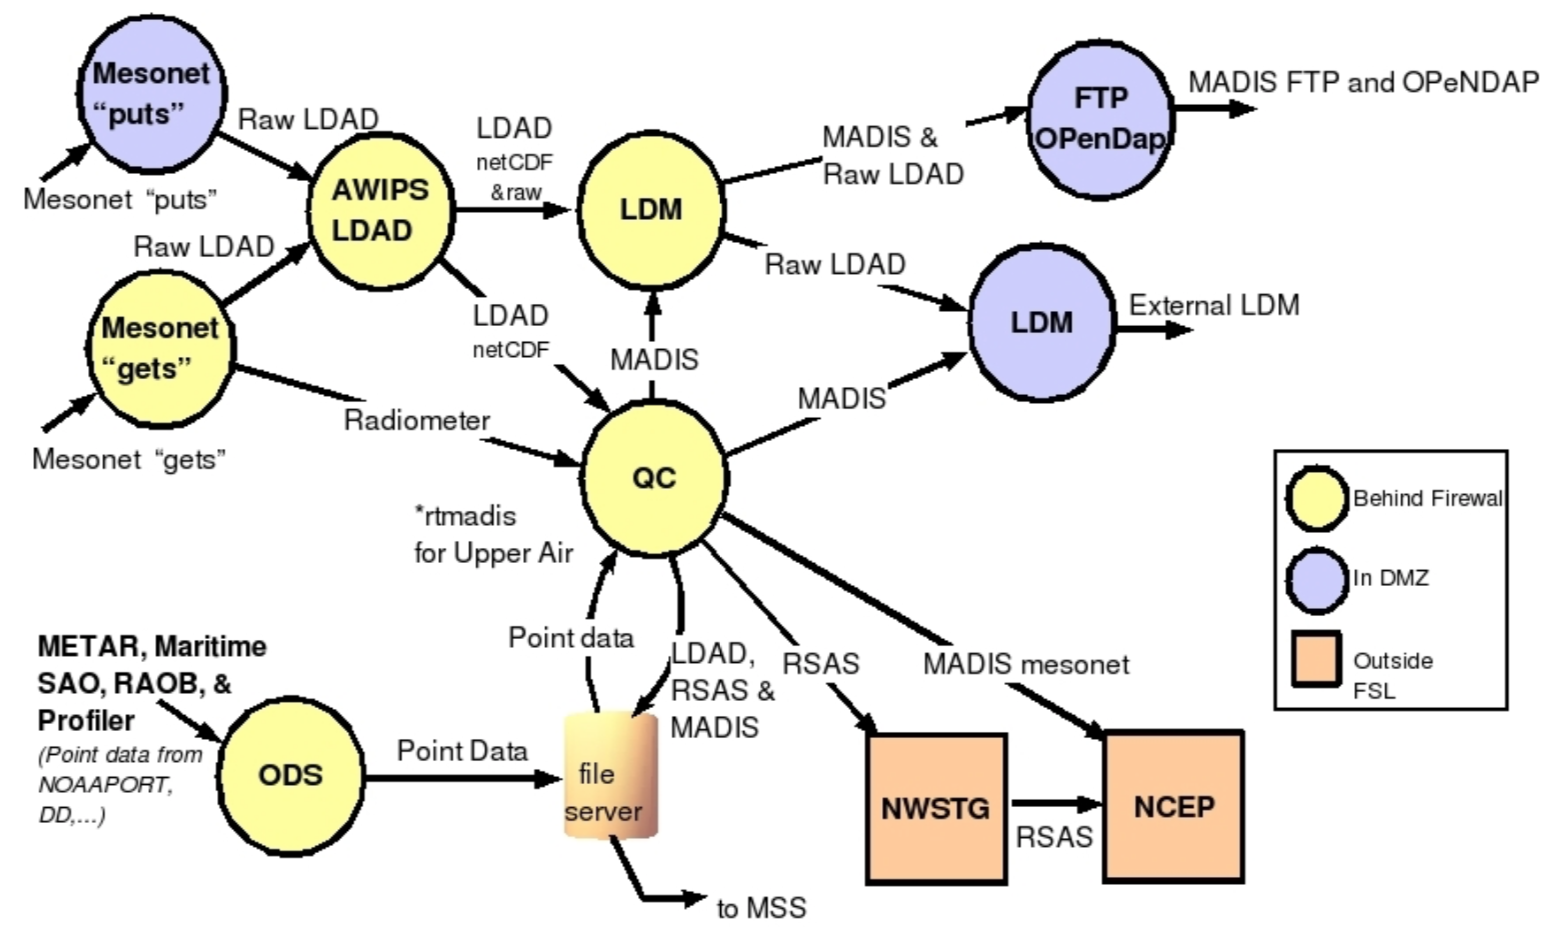
\includegraphics[width=1\textwidth]{lit/other/madis_flow.png}
    \caption[\acrshort{madis} flow]{\acrshort{madis} flow \cite{Macdermaid2005ARCHITECTUREP2.39}.}
    \label{fi:madis_flow}
\end{figure}

\acrshort{madis} comprises a distributed architecture for ingest, processing, and data distribution functions.
In addition, in a recent architectural advance, the various functional hosts are arranged in pairs using High-Availability (HA) Linux to provide auto mated failover in case of system failure. Real-time data distribution methods include FTP, Local Data Manager (LDM), and the Web-based OPeNDAP (OPen source project for Network Data Access Protocol) \cite{Macdermaid2005ARCHITECTUREP2.39}. As it mentioned above, the \acrshort{madis} is implemented based on a distributed architecture which is available at the time of it's development. Even it is not clear mentioned, it is using functional call like Remote procedure call (RPC) in order to invoke among a cluster of nodes as shown in figure \ref{fi:madis_flow}. In order to get High Availability, it has added some update to it's architecture. The conclusion of this statement is, these kind of functionalities are available at the modern the Cloud Computing tools, and out of the box those tools are providing the scalability and high availability. Using those tools, it possible to implement a such system with less effort and high confidence.

MADIS routinely acquires mesonet data from several dozen network providers representing over 14,000 stations. This translates into over 30,000 station reports each hour. Several systems running both inside and outside the firewall acquire the data. These data are sent to the Central Facility's Advanced Weather Interactive Processing System (AWIPS) data server for preprocessing and conversion to a common format, NetCDF. The NetCDF files are then transferred to the MADIS compute nodes \cite{Macdermaid2005ARCHITECTUREP2.39}. This provide an overview of the level of data that \acrshort{madis} handling. This could be a good reference for implementing \acrshort{wdias}, and it's performance testing. As same as \acrshort{fews}, it is also converting the data into a common format which is \acrshort{netCDF}. Those files are transferred to the computer nodes, and allow users to access via OPeNDAP.

The MADIS compute platforms comprise Intel based servers running the Red Hat Enterprise Linux operating system. Many of these computers are configured using High-Availability Linux clustering \cite{Macdermaid2005ARCHITECTUREP2.39}. As it indicated above, the system is heavily depend on the platform. There is a cost involving purchasing those license.

Since some MADIS data are considered proprietary by the provider, access to these data need to be controlled. To accommodate this, MADIS data are split into six different versions based on the level of access allowed by the data provider \cite{Macdermaid2005ARCHITECTUREP2.39}. When compared to \acrshort{fews}, \acrshort{madis} provide a control based access to the data.

\section{Summary}
\label{se:lit_summary}
